\documentclass[12pt]{article}

\usepackage{a4wide}
\usepackage[utf8]{inputenc}

\usepackage{graphicx}

%\pagestyle{empty}

\DeclareGraphicsRule{*}{mps}{*}{}
\begin{document}

\section*{Anisotropic Filtration}

\begin{figure}[ht]
    \centering
    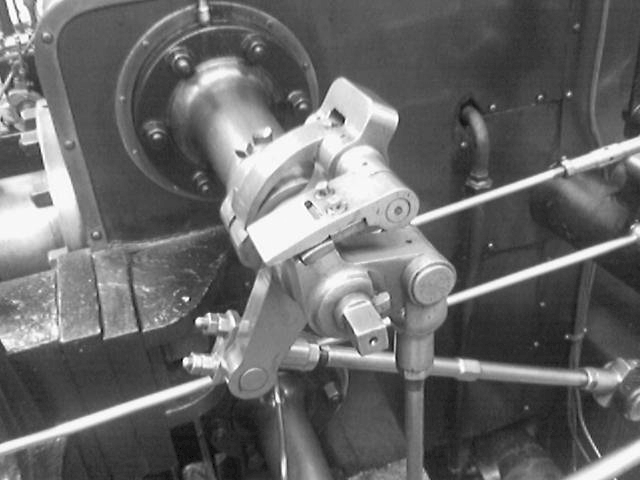
\includegraphics[width=0.45\textwidth]{input_image.png}
    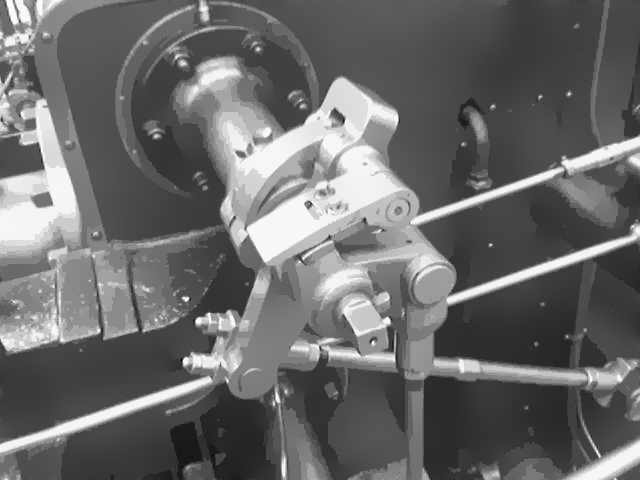
\includegraphics[width=0.45\textwidth]{anisotropic_filter_image.png}
    \caption{Input image (\textit{left} image); filtered image after 1000 iterations (\textit{right} image).}
\end{figure}

\noindent
Today's exercise is focused on the implementation of the anisotropic filtering of images.

\noindent
In contrast to the Gaussian blur, anisotropic filtration gives us filtered image that
still contains sharp edges. This filtration is based on simple physical phenomenon of
spreading an energy from higher concentrations to lower ones. In images, energy concentration
can be, for example, the brightness value in each pixel. All the pixels are placed in a grid
that forms a mesh network. Neighbour pixels are connected with each other by resistors
and their resistance (or conductance) is based on their similarity. The filtration then proceeds
in time. In each time step, small amounts of energy flows between pixels. After some predefined
number of time steps, the iteration stops.
\newline
\newline
\noindent
A model of a pixel neighborhood is depicted in Fig. \ref{fig:neighborhood}.
Conductances between pixels can be computed as follows

\begin{eqnarray} \label{eq:conduct}
    c_{N_{i,j}}^{t} &=& g \left(\left\|\nabla_N I_{i,j}^{t}\right\|\right) \nonumber \\
    c_{S_{i,j}}^{t} &=& g \left(\left\|\nabla_S I_{i,j}^{t}\right\|\right) \nonumber \\
    c_{E_{i,j}}^{t} &=& g \left(\left\|\nabla_E I_{i,j}^{t}\right\|\right) \nonumber \\
    c_{W_{i,j}}^{t} &=& g \left(\left\|\nabla_W I_{i,j}^{t}\right\|\right) \, ,
\end{eqnarray}
where $g$ is defined as follows

\begin{equation}
    g(\nabla I) = e^{\left(-\frac{\left| \nabla I\right|^2}{\sigma^2}\right)}
\end{equation}
and $\nabla_N I_{i,j} = I_{i-1,j} - I_{i,j}$. For other directions, it works the same way (see Fig. \ref{fig:neighborhood}).
\\
\\
\noindent
In each iteration step, a new value in a pixel is computed using the following formula

%\begin{eqnarray} \label{eq:iter}
%    I_{i,j}^{t+1} &=& I_{i,j}^{t} + \lambda \left[ c_N \cdot \nabla_N I + c_S \cdot \nabla_S I + c_E \cdot \nabla_E I + c_W \cdot \nabla_W I \right]_{i,j}^{t} \nonumber \\
%    &=& I_{i,j}^{t} \left( 1 - \lambda \left( c_N + c_S + c_E + c_W \right)_{i,j}^{t}\right) + \lambda \left( c_N \cdot I_N + c_S I_S + c_E I_E + c_W I_W \right)_{i,j}^{t} \, ,
%\end{eqnarray}

\begin{equation} \label{eq:iter}
    I_{i,j}^{t+1} = I_{i,j}^{t} + \lambda \left[ c_N \cdot \nabla_N I + c_S \cdot \nabla_S I + c_E \cdot \nabla_E I + c_W \cdot \nabla_W I \right]_{i,j}^{t} \, ,
\end{equation}
where $I_{i,j}^{t+1}$ is a new brightness value at coordinate $i,j$ at time $t+1$ and $I_{i,j}^t$ is an old brightness
value at coordinate $i,j$ at time $t$. Using the Eq. (\ref{eq:iter}) in each pixel, we compute new values at time $t+1$
based on the values at time $t$. Do not forget that this is not an in-place operation. You have to compute new values
to a new image.
\newline
\newline
Set $\sigma = 0.015$ and $\lambda = 0.1$ for your experiments.
\newline
\begin{figure}
    \centering
    \includegraphics[width=0.3\textwidth]{mpost/neighbours.1}
    \caption{A model of a pixel at coordinates $i,j$ with \textit{north} ($N$), \textit{south} ($S$), \textit{west} ($W$),
    and \textit{east} ($E$) neighbors.}
    \label{fig:neighborhood}
\end{figure}

\noindent
\textbf{Hint:} Use \texttt{double} data type to represent the input and output images.

%\section*{Expected Output}

\end{document}

